\section{Compact Sets}

\begin{exercise}
  Show that if $K$ is compact and nonempty, then sup $K$ and $\inf K$ both exist and are elements of $K$.
\end{exercise}

\begin{solution}
  Let $s = \sup K$, since $s$ is the least upper bound for every $\epsilon > 0$ there exists an $x \in K$ with $s - \epsilon < x$. Picking $\epsilon_n = 1/n$ and $x_n$ such that $s - \epsilon_n < x_n$ we get that $(x_n) \to s$ since $(\epsilon_n) \to 0$, and thus $s \in K$.

  A similar argument applies to $\inf K$.
\end{solution}

\begin{exercise}
  Decide which of the following sets are compact. For those that are not compact, show how Definition 3.3.1 breaks down. In other words, give an example of a sequence contained in the given set that does not possess a subsequence converging to a limit in the set.
  \enum{
  \item $\mathbf{N}$.
  \item $\mathbf{Q} \cap[0,1]$.
  \item The Cantor set.
  \item $\left\{1+1 / 2^{2}+1 / 3^{2}+\cdots+1 / n^{2}: n \in N\right\}$.
  \item $\{1,1 / 2,2 / 3,3 / 4,4 / 5, \ldots\} .$
  }
\end{exercise}

\begin{solution}
  \enum{
  \item Not compact, the sequence $x_n = n$ in $\mathbf N$ has no convergent subsequence in $\mathbf N$.
  \item Not compact, as we can construct a sequence $(x_n) \to 1/\sqrt 2 \notin \mathbf Q \cap [0, 1]$ implying $K$ is not closed, and thus cannot be compact.
  \item Compact, since the cantor set is bounded and closed since it is the infinite intersection of closed sets $\bigcap_{n=1}^\infty C_n$ where $C_1 = [0, 1/3] \cup [2/3, 1]$ etc where you keep removing the middle thirds of each interval.
  \item Not compact as every sequence $(x_n)$ contained in the set converges to $\pi^2/6$ which is not in the set, meaning the set isn't closed and thus cannot be compact.
  \item Compact since it is bounded and closed, with every sequence in the set converging to one.
  }
\end{solution}

\begin{exercise}
  Prove the converse of Theorem 3.3.4 by showing that if a set $K \subseteq \mathbf{R}$ is closed and bounded, then it is compact.
\end{exercise}

\begin{solution}
  Let $K$ be closed and bounded and let $(x_n)$ be a sequence contained in $K$. BW tells us a convergent subsequence $(x_{n_k}) \to x$ exists since $K$ is bounded, and since $K$ is closed $x \in K$. Thus every sequence in $K$ contains a subsequence convering to a limit in $K$, which is the definition of $K$ being compact.
\end{solution}

\begin{exercise}
  Assume $K$ is compact and $F$ is closed. Decide if the following sets are definitely compact, definitely closed, both, or neither.
  \enum{
  \item $K \cap F$
  \item $\overline{F^{c} \cup K^{c}}$
  \item $K \backslash F=\{x \in K: x \notin F\}$
  \item $\overline{K \cap F^c}$
  }
\end{exercise}

\begin{solution}
  \enum{
  \item Compact since $K \cap F$ is closed (finite intersection of closed sets) and bounded (since $K$ is bounded)
  \item Closed but not Compact since $K$ being bounded implies $K^c$ is unbounded, meaning $\closure{F^c \cup K^c}$ is unbounded.
  \item $K \setminus F = K \cap F^c$ could be either, if $K = [0,1], F^c = (0,1)$ then $K \cap F^c$ is open, but if $K = [0,1]$ and $F^c = (-1, 2)$ then $K \cap F^c = [0, 1]$ is compact.
  \item Compact since $K \cap F^c$ is bounded (since $K$ is bounded) implies $\closure{K \cap F^c}$ is closed (closure of a set is closed) and bounded (if $A$ is bounded then $\closure A$ is also bounded).
  }
\end{solution}

\begin{exercise}
  Decide whether the following propositions are true or false. If the claim is valid, supply a short proof, and if the claim is false, provide a counterexample.
  \enum{
  \item The arbitrary intersection of compact sets is compact.
  \item The arbitrary union of compact sets is compact.
  \item Let $A$ be arbitrary, and let $K$ be compact. Then, the intersection $A \cap K$ is compact.
  \item If $F_{1} \supseteq F_{2} \supseteq F_{3} \supseteq F_{4} \supseteq \cdots$ is a nested sequence of nonempty closed sets, then the intersection $\bigcap_{n=1}^{\infty} F_{n} \neq \emptyset$.
  }
\end{exercise}

\begin{solution}
  \enum{
  \item True, as it will be bounded and closed (since arbitrary intersections of closed sets are closed).
  \item False, $\bigcup_{n=1}^\infty [0, n]$ is unbounded and thus not compact.
  \item False, let $K = [0,1]$ and $A = (0,1)$. The intersection $K \cap A = (0,1)$ is not compact.
  \item False as $\bigcap_{n=1}^\infty [n, \infty) = \emptyset$ (It is true for compact sets though)
  }
\end{solution}

\begin{exercise}
  This exercise is meant to illustrate the point made in the opening paragraph to Section 3.3. Verify that the following three statements are true if every blank is filled in with the word ``finite.'' Which are true if every blank is filled in with the word ``compact''? Which are true if every blank is filled in with the word ``closed''?
  \enum{
  \item Every \blankk set has a maximum.
  \item If $A$ and $B$ are \blank, then $A+B=\{a+b: a \in A, b \in B\}$ is also \blank
  \item If $\left\{A_{n}: n \in \mathbf{N}\right\}$ is a collection of \blank sets with the property that every finite subcollection has a nonempty intersection, then $\bigcap_{n=1}^{\infty} A_{n}$ is nonempty as well.
  }
\end{exercise}

\begin{solution}
  \enum{
  \item Compact
  \item Closed, since if $a+b \in A+B$ then we can find sequences $(a_n) \to a$ and $(b_n) \to b$ in $A$ and $B$ respectively, with $(a_n + b_n)$ contained in $A+B$ and $(a_n + b_n) \to a+b$.
  \item Compact, since letting $K_n = \bigcap_{k=1}^n A_{k}$ gives $K_{n} \subseteq K_{n-1}$, we also have $K_n \ne \emptyset$ since every finite intersection is known to be nonempty. Applying the Nested Compact Set Property allows us to conclude
    $$
    \bigcap_{n=1}^\infty A_n = \bigcap_{n=1}^\infty K_n \ne \emptyset
    $$
  }
\end{solution}

\begin{exercise}
  As some more evidence of the surprising nature of the Cantor set, follow these steps to show that the sum $C+C=\{x+y: x, y \in C\}$ is equal to the closed interval $[0,2]$. (Keep in mind that $C$ has zero length and contains no intervals.)

  Because $C \subseteq[0,1], C+C \subseteq[0,2]$, so we only need to prove the reverse inclusion $[0,2] \subseteq\{x+y: x, y \in C\}$. Thus, given $s \in[0,2]$, we must find two elements $x, y \in C$ satisfying $x+y=s$
  \enum{
  \item Show that there exist $x_{1}, y_{1} \in C_{1}$ for which $x_{1}+y_{1}=s$. Show in general that, for an arbitrary $n \in \mathbf{N}$, we can always find $x_{n}, y_{n} \in C_{n}$ for which $x_{n}+y_{n}=s .$
  \item Keeping in mind that the sequences $\left(x_{n}\right)$ and $\left(y_{n}\right)$ do not necessarily converge, show how they can nevertheless be used to produce the desired $x$ and $y$ in $C$ satisfying $x+y=s$.
  }
\end{exercise}

\begin{solution}
  \enum{
  \item Define $2A = A+A = \{x+y : x,y \in A\}$, $C_1 = [0, 1/3] \cup [2/3, 1]$ has
    $$2C_1 = (2[0,1/3]) \cup (2[2/3, 1]) \cup ([0,1/3] + [2/3, 1])$$
    It's obvious that $2[0,1/3] = [0,2/3]$ and $2[2/3, 1] = [4/3, 2]$ now consider the last term, let $x \in [0,1/3]$ be fixed and let $y \in [2/3, 1]$ vary. obviously $x+y \in [2/3, 4/3]$ therefore adding the endpoints to compute $[0,1/3]+[2/3,1]=[2/3,4/3]$ works!
    % TODO: Rewrite this explanation at the top, unifying stupid 2*. and .+. notation for closed intervals

    This means that $2C_1 = [0,2/3] \cup [4/3, 2] \cup [2/3, 4/3] = [0, 2]$!

    \TODO Induction
  \item Since $C$ is compact, there exists a subsequence $(x_{n_k}) \to x$ with $x \in C$. Now since $x_{n_k} + y_{n_k} = s$ for all $k$, we have $\lim y_{n_k} = \lim s - x_{n_k} = s - x$. Now since each $y_{n_k} \in C$ the limit $y = s - x \in C$ as well, thus we have found $x,y\in C$ with $x+y = s$.
  }
\end{solution}

\begin{exercise}
  Let $K$ and $L$ be nonempty compact sets, and define
  $$
  d=\inf \{|x-y|: x \in K \text { and } y \in L\}
  $$
  This turns out to be a reasonable definition for the distance between $K$ and $L$.
  \enum{
  \item If $K$ and $L$ are disjoint, show $d>0$ and that $d=\left|x_{0}-y_{0}\right|$ for some $x_{0} \in K$ and $y_{0} \in L$.
  \item Show that it's possible to have $d=0$ if we assume only that the disjoint sets $K$ and $L$ are closed.
  }
\end{exercise}

\begin{solution}
  \enum{
  \item The set $|K - L| = \{|x-y| : x \in K, y \in L\}$ is compact since $K-L$ is compact by 3.3.6 (b) and $|\cdot|$ preserves compactness. Thus $d = \inf |K-L|$ has $d = |x_0 - y_0|$ for some $x_0 \in K$ and $y_0 \in L$.
  \item $K = \{n : n \in \mathbf N\}$ and $L = \{n + 1/n : n \in \mathbf N\}$ have $d = 0$, and both are closed since every limit diverges.
  }
\end{solution}


\begin{exercise}
  Follow these steps to prove that being compact implies every open cover has a finite subcover.

  Assume $K$ is compact, and let $\left\{O_{\lambda}: \lambda \in \Lambda\right\}$ be an open cover for $K$. For contradiction, let's assume that no finite subcover exists. Let $I_{0}$ be a closed interval containing $K$.
  \enum{
  \item Show that there exists a nested sequence of closed intervals $I_{0} \supseteq I_{1} \supseteq I_{2} \supseteq$ $\cdots$ with the property that, for each $n, I_{n} \cap K$ cannot be finitely covered and $\lim \left|I_{n}\right|=0$.
  \item Argue that there exists an $x \in K$ such that $x \in I_{n}$ for all $n$.
  \item Because $x \in K$, there must exist an open set $O_{\lambda_{0}}$ from the original collection that contains $x$ as an element. Explain how this leads to the desired contradiction.
  }
\end{exercise}

\begin{solution}
  \enum{
  \item Bisect $I_0$ into two intervals, and let $I_1$ be the interval where $I_1 \cap K$ cannot be finitely covered. Repating in this fashion we have $\lim |I_n| = \lim |I_0|(1/2)^n = 0$.
  \item The nested compact set property with $K_n = I_n \cap K$ gives $x \in \bigcap_{n=1}^\infty K_n$ meaning $x \in K$ and $x \in I_n$ for all $n$.
  \item Since $x \in O_{\lambda_0}$ and $|I_n| \to 0$ with $x \in I_n$ for all $n$, there exists an $N$ where $n > N$ implies $I_n \subseteq O_{\lambda_0}$ contradicting the assumption that $I_n \cap K$ cannot be finitely covered since $\{O_{\lambda_0}\}$ is a finite subcover for $I_n \cap K$.
  }
\end{solution}

\begin{exercise}
  Here is an alternate proof to the one given in Exercise 3.3.9 for the final implication in the Heine-Borel Theorem.

  Consider the special case where $K$ is a closed interval. Let $\left\{O_{\lambda}: \lambda \in \Lambda\right\}$ be an open cover for $[a, b]$ and define $S$ to be the set of all $x \in[a, b]$ such that $[a, x]$ has a finite subcover from $\left\{O_{\lambda}: \lambda \in \Lambda\right\}$.
  \enum{
  \item Argue that $S$ is nonempty and bounded, and thus $s=\sup S$ exists.
  \item Now show $s=b$, which implies $[a, b]$ has a finite subcover.
  \item Finally, prove the theorem for an arbitrary closed and bounded set $K$.
  }
\end{exercise}

\begin{solution}
  \enum{
  \item $S$ is nonempty since $x=a$ has the finite subcover $\{O_{\lambda_0}\}$ for $a \in O_{\lambda_0}$. $S$ is bounded since $x \le b$ for all $x \in S$.
  \item Suppose for contradiction that $s < b$, letting $s \in O_{\lambda_0}$ implies $[a,s]$ is finitely coverable since we can take the finite cover of an $x \in O_{\lambda_0}$ with $x < s$. This is causes a contradiction however since there exist points $y > s$ with $y \in O_{\lambda_0}$ meaning $[a,y]$ is also finitely coverable. therefore the only option is $s = b$, since any $s < b$ doesn't work.
  \item (a) still works, for (b) we must also consider the case where $y$ does not exist / there is a gap. Let $y = \inf\;[s, b]\cap K$ and suppose $y \ne s$. since $y \in [s,b] \cap K$ we know
    $$[a,y] \cap K = ([a,s]\cap K) \cup ((s, y]\cap K) = [a,s]\cap K \cup \{y\}$$
    therefore if $\{O_{\lambda_1}, \dots, O_{\lambda_n}\}$
    covered $[a, s]$ then letting $y \in O_{\lambda_{n+1}}$ would give the finite cover $\{O_{\lambda_1}, \dots, O_{\lambda_{n+1}}\}$ contradicting the assumption that $s < b$, therefore $s = b$ is the only option, and so $K$ can be finitely covered.
  }
\end{solution}

\begin{exercise}
  Consider each of the sets listed in Exercise 3.3.2. For each one that is not compact, find an open cover for which there is no finite subcover.
\end{exercise}

\begin{solution}
  \enum{
  \item $\mathbf{N}$ and $\{V_1(n) : n \in \mathbf{N}\}$ has no finite subcover since each $V_1(n)$ covers exactly one $n \in \mathbf{N}$, meaning there are no subcovers at all!
  \item $\mathbf{Q} \cap [0,1]$ and $\{O(x) : x \in \mathbf{Q}\cap[0,1]\}$ where $O(x) = V_{\frac 12|x-y|}(x)$ for $y \in \mathbf{Q}^c\cap [0,1]$ since any finite subcover $\{O(x_1), \dots, O(x_n)\}$ has $V_\epsilon(y) \notin O(x_i)$ for all $i$ when $\epsilon = \min_i\{\frac 12 |y - x_i|\}$. Thus the density theorem gives an $x \in V_\epsilon(y)$ with $x \in \mathbf{Q} \cap [0, 1]$ where $x$ is not in the finite cover.
    \TODO clean this up
  \item The Cantor is compact
  \item $K = \{1 + 1/2^2 + 1/3^2 + \dots + 1/n^2 : n \in \mathbf N\}$ and $\left\{V_{\frac 12 |x-L|}(x) : x \in K\right\}$ for $L = \pi^2/6$ since any finite cover $\left\{V_{\frac 12 |x_1-L|}(x_1), \dots, V_{\frac 12 |x_n-L|}(x_n)\right\}$, letting$\epsilon = \min\{\frac 12|x_i - L||\}$ will make $V_{\epsilon}(L)$ not in the finite cover, meaning there exists an $x \in V_\epsilon(L)$ with $x \in K$ (since $K$ gets arbitrarily close to $L$) but $x$ not in the finite cover.
  \item \{1, 1/2, 2/3, 3/4, 4/5, \dots\} is compact
  }
\end{solution}


\begin{exercise}
  Using the concept of open covers (and explicitly avoiding the Bolzano-Weierstrass Theorem), prove that every bounded infinite set has a limit point.
\end{exercise}

\begin{solution}
  Let $A$ be an infinite set bounded by $M$ (i.e. $|x|<M$ for all $x \in A$),
  suppose for contradiction that $A$ has no limit points,
  meaning there exists an $\epsilon > 0$ such that $V_\epsilon(x) \cap A = \{x\}$ for all $x \in A$.

  This immediately implies there are only a finite number of sets in our cover, otherwise the union would be unbounded. Contradiction.

  \TODO Finish tikz picture and proof (its visually obivous)

  \begin{figure}[!h]
    \centering
    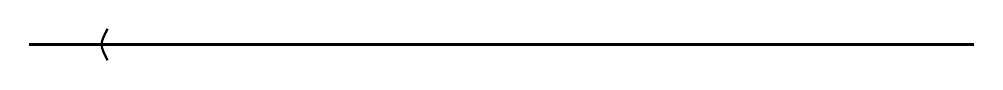
\begin{tikzpicture}
      \draw[thick] (-6,0) -- (6, 0);
      \draw[thick] (-5, 0.2) .. controls (-5.1, 0) .. (-5, -0.2);
      % \draw[thick, ->] (-5,0.2) arc (0:220:1);
    \end{tikzpicture}
  \end{figure}
\end{solution}

\begin{exercise}
  Let's call a set \emph{clompact} if it has the property that every \emph{closed} cover (i.e., a cover consisting of closed sets) admits a finite subcover. Describe all of the clompact subsets of $\mathbf{R}$.
\end{exercise}

\begin{solution}
  $K$ is clompact if and only if $K$ is finite, since the closed cover $\{[x,x] : x \in K\} = K$ having a finite subcover implies $\{[x,x] : x \in K\}$ is finite (since it is the only subcover that works) therefore $K$ is finite. If $K$ is finite then it obviously permits a finite subcover.
\end{solution}

